\section{Entwicklungsumgebung} \label{sec:tech-Entwicklungsumgebung}
\subsection{Eclipse}
Eclipse ist eine Open-Source-Framework, das meist als Entwicklungsumgebung genutzt wird und auf 11 verschiedenen Systemen und Architekturen verwendet werden kann. Darunter befinden sich unter anderem Windows, Linux, MAC OS X, etc. Eclipse ist der Nachfolger von Visual Age for Java von IBM. Der Quellcode von Eclipse wurde 2001 von IBM freigegeben. Eclipse bildet nur den Kern, die Funktionalit�t wird �ber Plug-ins realisiert. Je nach verwendeten Plug-ins stellt sich somit die gesamte Funktionalit�t der Entwicklungsumgebung zusammen. Sowohl Eclipse als auch die Plug-ins sind in Java implementiert. Die Plug-Ins sind teilweise frei verwendbar und teilweise kommerziell. Dabei werden neben Java auch andere Sprachen wie zum Beispiel: C, C++. Perl und PHP  unterst�tzt. Das dynamische Hinzuf�gen und Entfernen von Plug-ins und die daraus entstehende Gesamtfunktionalit�t der Eclipse-Entwicklungsumgebung bezeichnet man als Rich Client Platform, das wiederum auf den OSGi-Standard basiert.\\
Der OSGi-Standard (Open Services Gateway Initiative) ist ein Industriekonsortium, das ein  Framework, f�r die Vernetzung von intelligenten Embedded-Ger�ten und das Bereitstellen von Diensten zur Laufzeit erm�glicht, entwickelt hat. Eclipse verwendet das OSGi-Framework au�erhalb dieser Embedded-Ausrichtung.\\
F�r die GUI-Erstellung wurde in Eclipse SWT verwendet, da SWT auf die nativen GUI-Komponenten des jeweiligen Betriebssystems zugreift ist Eclipse, trotz Java, nicht als plattformunbh�ngig zu betrachten.\\
Der Aufbau von Eclipse setzt sich dabei aus folgenden Subsystemen zusammen, die teilweise aus einem oder mehreren Plug-ins bestehen wie in \vref{fig:eclipse-aufbau} zu sehen ist.
\begin{figure}[htbp]
	\centering
	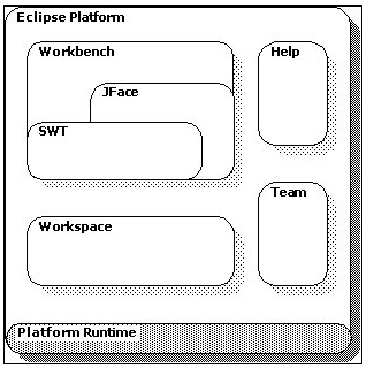
\includegraphics[scale=1.0]{images/Eclipse-Aufbau.png}
	\caption{Aufbau der Eclipse-Plattform}
	\label{fig:eclipse-aufbau}
\end{figure}
Die einzelnen Subsysteme definieren Erweiterungs-Schnittstellen um deren Funktionalit�t der Plattform zug�nglich zu machen, wie in Tabelle 3.1 auf Seite \pageref{tab:eclipse-subsystem} zu sehen ist. 

\begin{table}[htbp]
	\centering
	
\begin{longtable}{|c|p{10cm}|}
\caption{Subsysteme von Eclipse}\\

\hline
\textbf{Subsystem} & \textbf{Funktion} \endhead
\hline
Plattform-Runtime & Definiert die Erweiterungs-Schnittstellen und das Plug-in Model. Es findet dynamisch Plug-ins und enth�lt Informationen zu den Plug-ins und deren Schnittstellen in einem Register. Die eingef�gten Plug-ins werden gestartet, wenn der Anwender sie �ber die Plattform aufruft. \\
\hline
Resource Management & Definiert die API f�r das Erzeugen und Verwalten von Projekten, Dateien und Verzeichnissen, die von Tools erzeugt wurden und im Dateisystem abgelegt sind.\\
\hline
Workbench (UI) & Implementiert das Bedienfeld um mit der Plattform zu arbeiten. Definiert Erweiterungs-Schnittstellen f�r weitere UI-Komponenten, um vorhandene Funktionalit�ten aus bereits bestehenden Ansichten und Men�s zu erweitern oder zu verwenden. Als Grundlage dienen dazu JFace und SWT, die im Kapitel SWT beschrieben sind.\\
\hline
Help System & Definiert Erweiterungs-Schnittstellen f�r Plug-ins, um eine Hilfe oder andere Informationen als durchsuchbare B�cher bereitzustellen. \\
\hline
Team Support & Definiert ein Team-Programmierungsmodell zum Verwalten von Ressourcen. \\
\hline
Debug Support & Definiert ein sprachunabh�ngiges Debug-Modell und UI-Klassen f�r das Erstellen von Debuggern und Launchers.\\
\hline
Other Utilities & Andere n�tzliche Plug-ins unterst�tzen Funktionen f�r das Vergleichen von Ressourcen, das Erzeugen von Konfigurationen �ber XML-Files und das dynamische Updaten der Plattform �ber einen Server.\\
\hline
			
\end{longtable}
\label{tab:eclipse-subsystem}
\end{table}





\citep[Eclipse]{Wikipedia2005}
\citep{EclipseISV}



%Hier danach nicht mehr schreiben
\label{sec:tech-Entwicklungsumgebung-ende}